\documentclass[sigchi, review]{acmart}

\usepackage{booktabs} % For formal tables
\usepackage[utf8]{inputenc}
\usepackage{amsmath}
\usepackage{ wasysym }
\usepackage{tabularx}
\usepackage[german]{fancyref}
\usepackage[toc,page]{appendix}


% Copyright
\setcopyright{none}
%\setcopyright{acmcopyright}
%\setcopyright{acmlicensed}
%\setcopyright{rightsretained}
%\setcopyright{usgov}
%\setcopyright{usgovmixed}
%\setcopyright{cagov}
%\setcopyright{licensedcagov}
%\setcopyright{cagovmixed}
%\setcopyright{licensedothergov}

% DOI
%\acmDOI{10.475/123_4}

% ISBN
%\acmISBN{123-4567-24-567/08/06}

%Conference
%\acmConference[WOODSTOCK'97]{ACM Woodstock conference}{July 1997}{El
%  Paso, Texas USA}
%\acmYear{1997}
\copyrightyear{2018}

%\acmPrice{15.00}


\begin{document}
\title{Data Visualization: Potential Fields Method}
%\titlenote{Produces the permission block, and
%  copyright information}
%\subtitle{Extended Abstract}
%\subtitlenote{The full version of the author's guide is available as
 % \texttt{acmart.pdf} document}

% \author{Till-Julius Krüger}
% \affiliation{%
%   \institution{Freie Universität Berlin \\ Institut für Informatik}
% }
% \email{}

% \author{Michael Pluhatsch}
% \affiliation{%
%   \institution{Freie Universität Berlin \\ Institut für Informatik}
% }
% \email{}

% \author[3]{Anahid Roshandel}
% \affiliation{%
%   	\institution{Freie Universität Berlin \\ Institut für Informatik}
% }
% \email{}

% The default list of authors is too long for headers.
%\renewcommand{\shortauthors}{B. Trovato et al.}

%TODO Namen entfernen [x]
%TODO Kapitel umsortieren [x]
%TODO Quellen fuer verwendung [x]
%TODO Fußnote erste Seite entfernen [x]
%TODO Abstrakt überarbeiten [x]

\begin{abstract}
Dieses Paper beschäftigt sich mit der Analyse und Planung einer Visualisierung der \textit{Potential Fields Method} für Studierende des ersten Semesters und Interessierte nach dem Abitur. Dafür haben wir  verschiedene vorhandene Ansätze betrachtet und analysiert. Aus den resultierenden Erkenntnissen haben wir einen eigenen Prototyp erstellt. Dieser erschafft zunächst mit dem Blackbox-Verfahren ein Verständnis für das Problem des Algorithmus. Danach sollen mit Hilfe des Whitebox-Verfahrens Einblicke in die Funktionsweise des Algorithmus gewährt werden. Nach der Implementierung soll die Visualisierung evaluiert werden.
\end{abstract}


\keywords{Potential Fields Method, Data Visualization, Analyse, Algorithmus}

\begin{teaserfigure}
  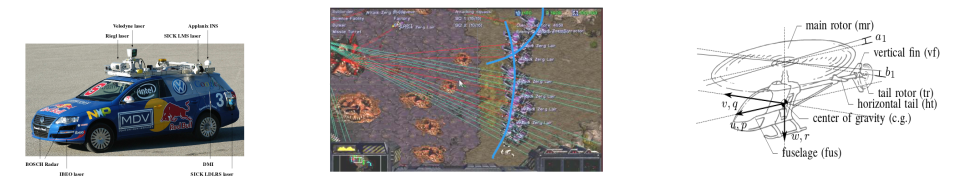
\includegraphics[width=\textwidth]{img/teaser}
  \caption{Anwendungsmöglichkeiten der \textit{Potential Field Method}~\cite{hagelback2012potential}\cite{montemerlo2008junior}\cite{paul2008uav}}
  \label{fig:teaser}
\end{teaserfigure}


\maketitle

% =============================================================================
\section{Problembeschreibung und Eignung des Algorithmus}\label{sec:intro}
% =============================================================================

Der \textit{Potential Fields Method} Algorithmus befasst sich grundlegend mit der Pfadplanung eines Roboters. Das Problem besteht dabei aus einem Roboter, der sich zu einem Ziel bewegen soll. Die Pfadplanung versucht einen Pfad vom Startpunkt des Roboters zum Ziel zu planen. Dabei sollen Kollisionen mit Hindernissen vermieden werden. Der Pfad sollte außerdem so kurz wie möglich sein.

Im Falle der \textit{Potential Fields Method} werden hierfür einfache physikalische Gesetze verwendet. Bei der Pfadplanung werden künstliche Kräfte bzw. Potentiale berechnet, die den Roboter zum Ziel weisen. Der Roboter wird vom Potentialfeld des Ziels angezogen, aber vom Potentialfeld des Hindernisses abgestoßen. Die Kräfte werden mit einigen Gleichungen berechnet, die in Abschnitt \vref{sec:algo} erläutert werden.

Der Algorithmus behandelt ein abstraktes Problem, das auch ohne jegliche Vorkenntnisse verständlich ist. Daher ist er für Erstsemesterstudierende ohne fundiertes Wissen möglich zu verstehen. Man braucht lediglich mathematisches und physikalisches Verständnis aus dem Abitur. 
Für Erstsemesterstudierende könnte der Algorithmus für die Mathematik im Studium motivieren, da es ein mathematisches Konstrukt entmystifiziert. Scheinen die mathematischen Gleichungen im ersten Moment erschlagend, können sie durch eine gute Visualisierung Schritt für Schritt erschlossen werden. 

Durch die variierbare Komplexität und mögliche Erweiterungen ist der Algorithmus aber auch für fortgeschrittene Studenten von Interesse. 
Der Algorithmus wird im Modul \textit{Robotik} gelehrt und wird auch in der modernen Forschung noch verwendet. Beispiele sind hier autonome Automobile~\cite{dolgov2009path}, Computerspiele wie Starcraft~\cite{hagelback2012potential}, Drohnen~\cite{paul2008modelling} und Mars-Rover~\cite{massari2004autonomous}. Die ersten drei Beispiele sind in Abbildung~\vref{fig:teaser} abgebildet.
%-> Abstraktes Problem, leicht verständlich, ohne Vorkenntnisse
%-> Variierbare Komplexität (Erweiterungen etc)
%-> Einfache Mathemathik, Abiturwissen
%-> Motivation fuer Mathemathik im Studium


% =============================================================================
\section{Algorithmus}\label{sec:algo}
% =============================================================================

Der Algorithmus \textit{Potential Fields Method} nutzt einfache physikalische Elemente zur Vermeidung von Kollisionen mit einem Hindernis.

\subsection{Beschreibung}
Es wird eine Kraft $F$ beschrieben, welche die Bewegung des Roboters beeinflusst um das Ziel zu erreichen und Hindernissen auszuweichen.
Diese Kraft besteht dabei aus zwei Komponenten, die für jede Konfiguration $q$ berechnet werden kann.
Hierbei stellt $q$ eine Konfiguration im Konfigurationsraum dar (zum Beispiel eine $xy$ Koordinate).
Eine Konfiguration ist eine Position, die der Roboter anfahren kann.
Der Konfigurationsraum enthält alle anfahrbaren Konfigurationen.
Der Roboter hat dabei die Konfiguration $q_r$.
In jeder Iteration des Algorithmus wird eine neue Position des Roboter berechnet:
\begin{equation}
	q_r = \sigma \cdot \frac{F(q_r)}{|F(q_r)|}
\end{equation}
Hierbei bezeichnet $\sigma$ die Schrittweite des Roboters. Das bedeutet, dass dieser Parameter enscheidet, wie weit sich der Roboter in Richtung der berechneten Kraft $F(q_r)$ bewegt. Aus diesem Grunde wird die $F(q_r)$ normalisiert, sodass nur $\sigma$ die Schrittweite beeinflusst.

$F(q_r)$ wird aus zwei Termen berechnet:
\begin{equation} \label{eq:grad_field}
     F(q_r) = F_{\text{anziehend}}(q_r, q_z) + F_{abstoßend}(q_r,q_h)
\end{equation}
Unter $F_{\text{anziehend}}(q_r, q_z)$ versteht sich eine anziehende Kraft, die den Roboter in  Richtung einer Position leitet.
Dies ist das Ziel des Roboters.
Dadurch wird dafür gesorgt, dass der Roboter sich in Richtung des Ziels $q_z$ bewegt.
Hierfür gibt es verschiedene Variationen, die hier beschriebene Variante nennt sich \textit{konisch} \cite{Formulars}.
\begin{equation}\label{eq:grad_attr}
	F_{\text{anziehend}}(q_r, q_z)= -U_{\text{anziehend}}(q_r, q_g) \cdot (q_r - q_z)
\end{equation}

\begin{equation}\label{eq:pot_attr}
	U_{\text{anziehend}}(q_r, q_z) = - \epsilon \cdot \frac{1}{\lvert\lvert q_r - q_z \rvert\rvert}
\end{equation}
Es wird ein Vektor in Richtung des Ziels bestimmt und mit dem Potential $U_{\text{anziehend}}(q_r, q_z)$ gewichtet. Dabei gibt es den Parameter $\epsilon$, mit dem die anziehende Kraft verstärkt oder abgeschwächt werden kann.
\newline
Nutzt man nur die anziehende Kraft $F_{\text{anziehend}}(q_r, q_z)$, bewegt sich der Roboter zwar zum Ziel, ignoriert auf seinem Weg allerdings jegliche Hindernisse.
Um dem entgegen zu wirken, geht auch von den Hindernissen eine Kraft aus: $F_{\text {abstoßend}}(q_r, q_h)$.
Diese wird für das Hindernis mit dem kleinsten Abstand $p(q_r)$ mit Konfiguration $q_h$  berechnet:
\begin{equation}\label{eq:grad_rep}
	F_{\text{abstoßend}}(q_r, q_h) =
	\begin{cases}
    [0,0] ,& \text{if } \phi > p(q_r)\\
    U_{\text{abstoßend}}(q_r, q_h) \cdot (q_r-q_h),               & \text{otherwise}
\end{cases}
\end{equation}

\begin{equation}\label{eq:pot_rep}
     U_{\text{abstoßend}} = \theta \cdot U_{\text{Erkennung}} \cdot U_{\text{Entfernung}} \cdot \frac{1}{ \lvert q_r - q_o \rvert }
\end{equation}
\begin{equation}
 U_{\text{Erkennung}} = \left( \frac{1}{\lvert p(q_r) \rvert} - \frac{1}{\phi} \right)
\end{equation}
\begin{equation}
U_{\text{Entfernung}} = \frac{1}{p(q_r)^2}
\end{equation}

\begin{figure}
  \centering
  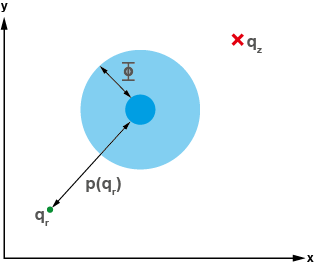
\includegraphics[width=0.7\linewidth, height=0.7\linewidth]{img/Params}
  \caption{Darstellung der Parameter des Algorithmus.}
  \label{fig:params}
\end{figure}

Das bedeutet, dass die abstoßende Kraft nur angewandt wird, wenn $p(q_r) \leq \phi$ ist. 
Dann wird wieder ein Richtungsvector bestimmt und mit dem Potential $U_{\text{abstoßend}}(q_r, q_h)$ gewichtet.
Dadurch beginnt der Roboter dem Hindernis erst auszuweichen, wenn der Grenzwert $\phi$ überschritten wird.
Der Roboter erkennt also Hindernisse in einem Abstand von $\phi$.
Durch dieses Verhalten soll ein kürzerer Weg zum Ziel erreicht werden.

$\theta$ ist hier das Äquivalent von $\epsilon$ für Hindernisse. 
Es dient zur allgemeinen Veränderung der abstoßenden Kraft.
Mit $U_{\text{Erkennung}}$ wird die Stärke der Kraft relativ zu einer Grenze $\phi$ bestimmt.
Der letzte Term $U_{\text{Entfernung}}$ skaliert die Kraft im Verhältnis zur Entfernung des Hindernisses. Je näher es ist, desto stärker wird die abstoßende Kraft.

Die einzelnen Parameter sind in Abbildung~\vref{fig:params} verdeutlicht.


\subsection{Verständnisschwerpunkte}
Aus persönlicher Erfahrung liegt die Schwierigkeit beim Verständnis des Algorithmus bei den mathematischen Gleichungen, die das Zusammenspiel der Kräfte beschreiben.
Werden nur die Gleichungen ohne ein anschauliches Beispiel betrachtet, erscheinen die Gleichungen abstrakt und  komplex.
Daher sollen die Gleichungen in die einzelnen Terme aufgebrochen werden.
Durch eine Visualisierung sollen die Auswirkungen der Veränderung einzelner Terme sichtbar gemacht werden.
Auf diesem Wege wird immer nur ein Teil der Gleichung betrachtet und sich dessen Veränderung bewusst gemacht.
Durch diese Möglichkeit zum Experimentieren soll die Mathematik interaktiv verstanden werden. 

\section{Verwandte Arbeiten}

Wir haben verschiedene Visualisierungsmöglichkeiten gefunden.

\subsection{Beschreibung}
\begin{itemize}
\item Abbildung~\vref{fig:other_pyrob}  ist ein Ausschnitt einer Animation, die den Weg des Roboters zeigt. Die Darstellung verwendet eine Farbkarte zur Visualisierung der Kraft. Durch die Farbintensität wird verdeutlicht, welche Kraft an welcher Konfiguration herrscht. Ein dunkler Farbwert steht für ein hoch abstoßenden Kraftwert, helle Werte sind hingegen anziehend. Daher sind die Hindernisse sowie Bereiche hinter dem Roboter sehr dunkel, das Ziel jedoch sehr hell. Durch den Farbverlauf kann eine Richtung erkannt werden, in die der Roboter forciert wird. Der Roboter bewegt sich entlang der roten Linie vom Startpunkt zum Ziel. Die Eingabedaten und Parameter des Algorithmus sind hier nicht veränderbar.
\item Bei Abbildung~\vref{fig:other_mcgill} wird die Kraft jeder Konfiguration als Vektor in jeder möglichen Konfiguration dargestellt. Aus diesem Grund zeigen die Pfeile (Vektoren) vom Hindernis fort und in Richtung des Ziels. Der Kreis in Magenta stellt das Ziel dar, während das Hindernis durch einen grünen Kreis symbolisiert wird. In dieser Visualisierung ist der Einfluss von $\phi$ gut erkennbar, da der Einflussbereich des Hindernisses sich kreisförmig um das Hindernis ausbreitet.
\item Das letzte Beispiel (Abbildung~\vref{fig:other_elec}) zeigt ein verwandtes Thema. Es behandelt elektronische Felder. Diese entwickeln auch ein Kräfteverhältnis und visualisieren somit ein ähnliches Problem. Der grüne Kreis wird von den roten Kreisen angezogen. Die roten Kreise stoßen sich hingegen ab. Daher könnte der Roboter als grüner Kreis verstanden werden und rote Kreise als Ziele.
\end{itemize}

\begin{table*}[b]
  \centering
  \begin{tabularx}{\textwidth}{l|l|c|c|c}
   Kategorie & Kriterium  & \cite{PythonRobotics} & \cite{McGill} & \cite{Electric} \\\hline
   Interaktivität & Objekte verschiebbar &\lightning & \lightning & \checked \\
   Interaktivität & Verhalten änderbar & \lightning & \lightning & \checked \\
   Erklärbarkeit & Erklärender Text vorhanden & \checked \lightning  wenig & \checked & Link Wikipedia\\
   Erklärbarkeit & Überschrift / Unterschrift vorhanden & \checked & \checked & \checked \\
   Erklärbarkeit & Achsenbeschriftung vorhanden & (\checked) \lightning & (\checked) \lightning & \lightning\\
   Erklärbarkeit & Legende vorhanden & \lightning & \lightning & \checked \\
   Erklärbarkeit & Selbsterklärend & \checked & \checked \lightning & \checked \lightning\\  
   Erklärbarkeit & Statisch/Dynamisch & Dynamisch & Statisch & Dynamisch \\
   White/Blackbox & Einblick in Algorithmus & & & \checked \\
   White/Blackbox & Algorithmus verständlich & \checked & \checked & \lightning \\
   White/Blackbox & Probleminformation & & \lightning & \lightning \\
     
\end{tabularx}
  \caption{Morphologische Analyse}
  \label{tab:morph}
\end{table*}

\subsection{Analyse}
Wir haben auf den beschriebenen Beispielen eine morphologische Analyse (Tabelle~\vref{tab:morph}) durchgeführt. Daraus ließen sich die folgenden Erkenntnisse ableiten.
\begin{itemize}
    \item Abbildung~\vref{fig:other_pyrob}: Die Visualisierung versucht, den Weg des Roboters zu erklären, indem die Kräfte der möglichen Konfigurationen zu jedem Zeitpunkt durch die Farbkarte sichtbar sind. Dadurch erhält der Nutzer ein Verständnis, warum der Roboter den zurückgelegten Weg gewählt hat. Der Nutzer muss dafür aber die gesamte Welt des Roboters im Blick haben, was im ersten Moment überfordernd wirkt. Das Verständnis wird daher nicht Schritt für Schritt aufgebaut und ist eher für fortgeschrittene Betrachter geeignet.
    \item Abbildung~\vref{fig:other_mcgill}: Auch bei dieser Visualisierung wird das globale Kräftewirken verdeutlicht. Allerdings wird hier ein Vektorfeld benutzt. Die Vor- und Nachteile der vorherigen Abbildung sind jedoch auch hier zu finden. 
    \item Abbildung~\vref{fig:other_elec}: Der Vorteil dieser Visualisierung ist ein sehr klarer, einfacher Aufbau. Es wird nicht versucht, die wirkenden Kräfte des ganzen Feldes an jedem Punkt zu visualisieren. Dadurch ist die Visualisierung weniger überladen. Es bleibt überschaubarer und überfordert den Betrachter nicht. Allerdings stellt es unseren Algorithmus nicht exakt dar, es gibt kein Äquivalent für Hindernisse.
\end{itemize}

Als Folge daraus werden wir versuchen, die Whitebox-Darstellungen (globale Farbkarte aus Abbildung~\vref{fig:other_pyrob}, lokale Vektordarstellung aus Abbildung~\vref{fig:other_mcgill}) in einer separaten Ansicht zu zeigen. 
Wir finden dabei die Ansicht aus ~\vref{fig:other_pyrob} intuitiver. 
Dabei sollen nur die wirkenden Kräfte gezeigt werden und der Roboter, die Hindernisse und das Ziel in einer eigenen Ansicht dargestellt werden.
Wir möchten die Darstellung jedoch noch um eine zusätzliche Dimension erweitern und die Stärke der Kraft nicht nur durch Farbe, sondern auch durch Höhe kodieren.

In der Roboter-Ansicht wollen wir die klare Einfachheit und hohe Interaktivität aus Abbildung~\vref{fig:other_elec} für unsere Visualisierung nutzen. Dadurch kombinieren wir alle Vorteile der bestehenden Visualisierungen auf eine neue Art.
Durch diese Aufteilung soll der Nutzer Schritt-für-Schritt an das Problem und den Algorithmus herangeführt werden, ohne ihn zu überfordern.

\begin{figure}
  \centering
  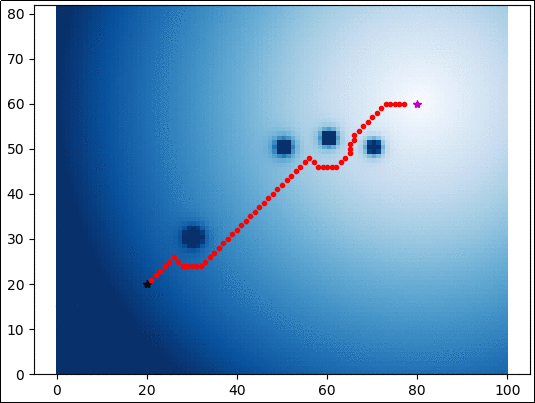
\includegraphics[width=0.7\linewidth, height=0.7\linewidth]{img/pythonrobotics}
  \caption{Beispielhafte Visualisierung mit einer Farbkarte~\cite{PythonRobotics}.}
  \label{fig:other_pyrob}
\end{figure}

\begin{figure}
\label{mcg}
  \centering
  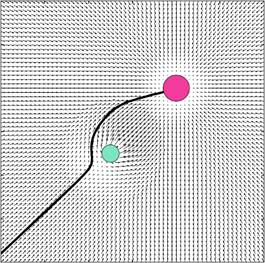
\includegraphics[width=0.7\linewidth, height=0.7\linewidth]{img/mcgill}
  \caption{Beispielhafte Visualisierung als Vektorfeld~\cite{McGill}.}
  \label{fig:other_mcgill}
\end{figure}
\begin{figure}
  \centering
  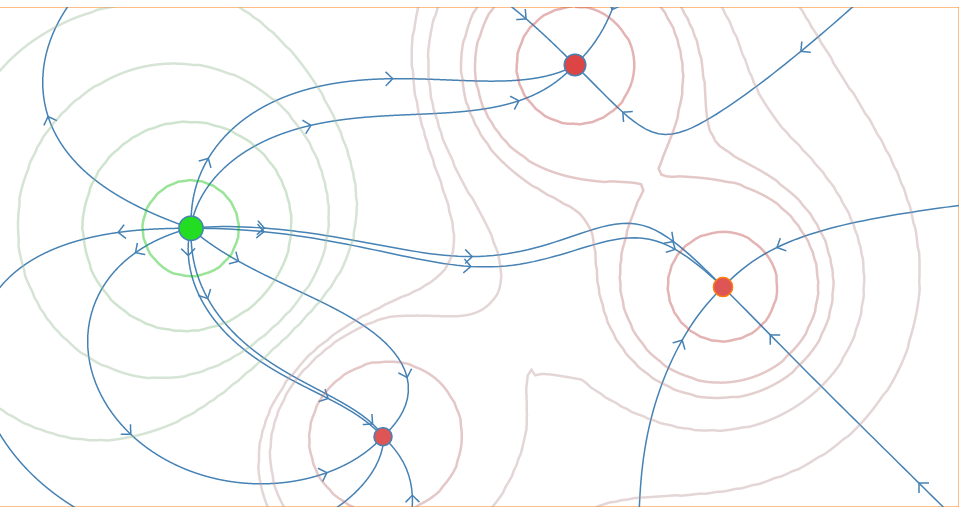
\includegraphics[width=0.7\linewidth, height=0.7\linewidth]{img/electric2}
  \caption{Interessante Visualisierung für elektronische Felder~\cite{Electric}.}
  \label{fig:other_elec}
\end{figure}

% =============================================================================
\section{Ansatz/Prototyp} \label{sec:prot}
% =============================================================================

% Begriffe definieren!!!!
Zunächst wird dem Nutzer in einer Einleitung das Problem der Pfadplanung erläutert. Konkret, wie kommt zum Beispiel ein Roboter von seinem Startpunkt zu einem Ziel. Die Studenten und Studentinnen bekommen ein allgemeines Verständnis für Pfadplanungen und deren Anwendungen. Gleichzeitig wird ihnen vermittelt, welche Probleme bei einer Pfadplanung auftreten können. So müssen zum Beispiel kürzeste Wege gefunden, Hindernisse umgangen und Sackgassen gemieden werden. Anschließend wird mit der sogenannten \textit{Potential Fields Method} eine Lösung vorgestellt. Die Hauptzielgruppe in diesem Projekt sind Erstsemesterstudierende im Fach Informatik. Jedoch wird der Algorithmus auf unterschiedliche Art und Schwierigkeit erklärt, so dass auch fachfremde Personen ein einfacher Einstieg in die Thematik gegeben werden soll. 


\begin{figure}[ht!]
  \centering
  \fbox{
  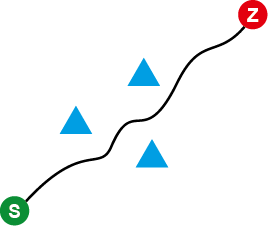
\includegraphics[width=0.7\linewidth, height=0.7\linewidth]{img/statischBB}}
  \caption{Abstrakte, statische Darstellung des Problems}
  \label{fig:bbstatic}
\end{figure}


%TODO Einleitung die die Abschnitte/Gliederung erklaert
Mit der ersten Visualisierung wird der Algorithmus allgemein vorgestellt und anhand einer Animation gezeigt. % und zur Problemerklärung!
Abbildung~\vref{fig:bbstatic} stellt dafür ein Beispiel dar.  Dabei wird ein Roboter (bzw. ein Startobjekt) gezeigt, der sich in Richtung Ziel bewegt und die Hindernisse umgeht. Der zurückgelegte Weg wird nach und nach eingeblendet. Die Animation kann nicht verändert werden. Um die Animation zu steuern, gibt es einen Start- und Stoppknopf. Neben der Animation wird das Problem mit Text vorgestellt. % Zuerst das Problem
\begin{figure}[ht!]
  \centering
  \fbox{
  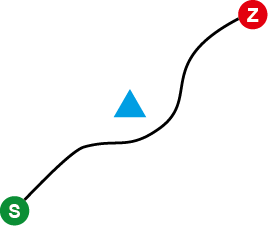
\includegraphics[width=0.7\linewidth, height=0.7\linewidth]{img/interaktiv}}
  \caption{Interaktiv veränderbares Beispiel}
  \label{fig:interaktiv}
\end{figure}


Für die Erklärung des Algorithmus benutzen wir zwei Ansätze. Der erste Ansatz beruht auf dem sogenannten Blackbox Verfahren. Das heißt, dass der Nutzer  Eingaben verändern kann und  ein entsprechendes Ergebnis erhält ohne die genauen Abläufe des Algorithmus zu kennen. Wir möchten den Nutzer spielerisch an die \textit{Potential Fields Method} heranführen und ihn für den Algorithmus begeistern. Der Nutzer bekommt die Möglichkeit interaktiv mit den Objekten zu spielen. Die Abbildung enthält ein Start- und Zielobjekt und ein Hindernis, wie in Abbildung~\vref{fig:interaktiv} dargestellt. Durch das Verschieben des Start- und Zielpunkts und das Setzen von Hindernissen wird dem Nutzer visuell und interaktiv vermittelt, wie sich der Algorithmus verhält und wie die Auswirkungen auf die Pfadplanung sind. Der Fokus im ersten Teil des Ansatzes liegt darin, allen Personengruppen die Thematik visuell zu erklären und eine Einführung zu geben.


\begin{figure}[ht!]
  \centering
  \fbox{
  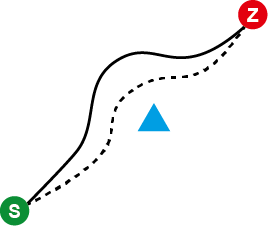
\includegraphics[width=0.7\linewidth, height=0.7\linewidth]{img/Whitebox}}
  \caption{Whitebox Beispiel mit veränderbaren Parametern}
  \label{fig:whitebox}
\end{figure}

\begin{figure}[ht!]
  \centering
  \fbox{
  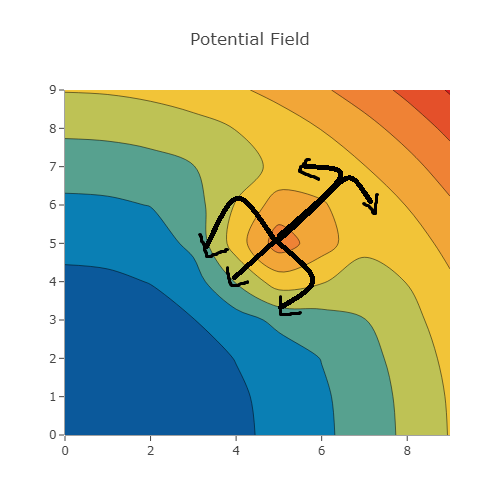
\includegraphics[width=0.7\linewidth, height=0.7\linewidth]{img/contourPfeil.png}}
  \caption{Kräfte dargestellt als Isokonturen und lokalen Flussgraphen}
  \label{fig:isocon}
\end{figure}

\begin{figure}[ht!]
  \centering
  \fbox{
  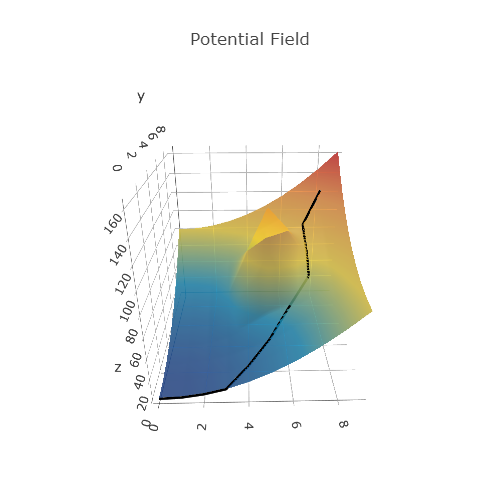
\includegraphics[width=0.7\linewidth, height=0.7\linewidth]{img/3dfield.png}}
  \caption{3D Visualisierung der Kräfte mit Pfad}
  \label{fig:3dmountain}
\end{figure}

Mit dem zweiten Ansatz, unter Zuhilfenahme des sogenannten Whitebox Verfahrens, verfolgen wir die Vermittlung eines tiefgründigen Verständnisses des Algorithmus. Der Fokus dieser Erklärung richtet sich an fachnahe Personen, speziell Erstsemesterstudierende. Hier wird dem Nutzer mit vorgegebenen Eingaben detailliert der Algorithmus erklärt. Es können Parameter mithilfe von Reglern verändert werden. In Abbildung~\vref{fig:whitebox} wird ein Weg in gestrichelter Linie gezeigt, welcher einem Standardweg entspricht.
Werden Parameter verändert, so wird im Vergleich zum Standardweg ein neuer Weg mit den veränderten Parametern berechnet und gezeigt. Die Positionen der Objekte kann jedoch nicht verschoben werden, da es bei dieser Erklärung in erster Linie um die Auswirkungen der Parameter geht.
Mit den Parametern werden die anziehenden und abstoßenden Kräfte verändert und visuell dargestellt. Dabei haben wir uns gegen die klassische Darstellung mit Vektorfeldern entschieden (Abbildung~\vref{fig:other_mcgill}). Ungeübte Betrachter können nur schwer erkennen wie  nicht zirkulierende Senken und Quellen \cite{munzner2015visualization} interagieren. Es ist nicht intuitiv ersichtlich wie bzw. wo ein Weg für die Pfadfindung entsteht. Ebenso  verhält es sich mit den in Abbildung~\vref{fig:other_elec} dargestellten elektronischen Feldern. Für ein besseres Verständnis haben wir  einerseits eine aktivierbare und deaktivierbare Darstellung mit Isokonturen \cite{munzner2015visualization} und lokale Vektoren gewählt. Dabei stellen die unterschiedlichen Farben die anziehenden bzw. abstoßenden Kräfte dar, welche mit den lokalen Vektoren hervorgehoben werden (Abbildung~\vref{fig:isocon}). Andererseits wird diese Darstellung mit einer 3D Karte anschaulich erklärt. Die unterschiedlichen Farben repräsentieren hierbei verschiedene Höhenmeter. Objekte mit abstoßenden Kräften werden als Berge visualisiert und das Ziel mit der anziehenden Kraft als Tal. Ziel des Roboters ist ein möglichst schneller und einfacher Weg ins Tal (Abbildung~\vref{fig:3dmountain}). Dies ist vergleichbar mit einem Ball der ins Tal rollt.



Nachdem der Nutzer ein grundlegendes Verständnis über den Algorithmus vermittelt bekommen hat, möchten wir auf potenzielle Probleme hinweisen, wie z. B. in Abbildung \vref{fig:pfprob}. Dort sieht man, dass der Roboter in ein lokales Minimum geraten ist und dieses nicht mehr verlassen kann. Zum Schluss zeigen wir, dass der vorgestellte Algorithmus nicht nur ein theoretisches Konstrukt ist. Anhand von realen Beispielen wird der praktische Nutzen belegt (siehe Abschnitt~\vref{sec:intro}).%Hallo Micha!

\begin{figure}[ht!]
  \centering
  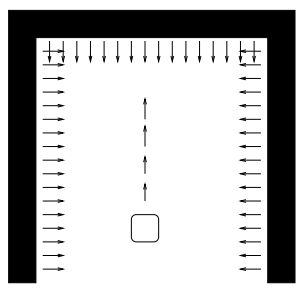
\includegraphics[width=0.7\linewidth, height=0.7\linewidth]{img/pfprob}
  \caption{Box Canyon Problem~\cite{Goodrich2002PotentialFT}.}
  \label{fig:pfprob}
\end{figure}

%\subsection{Prototyp}



%2) Im nächsten Schritt bekommt der Nutzer die Möglichkeit mit den Objekten zu spielen. % spielerisch das Problem/ALgo kennen zu leren?
%Das interaktive Bild enthält ein Start- und Zielobjekt und ein Hindernis, wie in Bild~\vref{fig:interaktiv} dargestellt. Alle Objekte können verschoben werden und es können auch gegenbenenfalls neue Hindernisse hinzugefügt werden. Dementsprechend wird der neue Pfad gezeigt. Der Nutzer bekommt aber nur eine Blackbox gezeigt, das dieser zwar die Objekte bewegen kann, aber nicht gezeigt wird, wir der Algorithmus den Pfad findet. % Geschlechtzeug? Was ist eine BB - Begriff definieren

%3) Im dritten Abschnitt bekommt der Nutzer einen Einblick in die Whitebox. %Begriff definieren
%Hier können die Parameter mit Hilfe von Reglern verändert werden. In Bild~\vref{fig:whitebox} wird ein Weg in gestrichelter Linie gezeigt, welcher einem Default Weg entspricht. 
%Im Vergleich dazu wird ein Weg mit den neuen  veränderten Parameter berechnet und gezeigt. Man kann hier allerdings die Position der Objekte nicht verschieben, da es hier in erster Linie um die Parameter geht.

%4) Im vierten Abschnitt werden die anziehenden und abstoßenden Kräfte visuell dargestellt. Dabei haben wir uns gegen die klassische Darstellung mit Flussgraphen für Vektor Feldern entschieden (Bild~\vref{fig:mcgill}). Ungeübte Betrachter können nur schwer erkennen wie  nichtzirkulierende Senken und Quellen interagieren und wie bzw. wo ein Weg für die Pfadfindung entsteht. Ebenso  verhält es sich mit den in Bild~\vref{fig:elec} dargestellten elektronischen Feldern. Für ein besseres Verständnis haben wir  einerseits eine Darstellung mit Isokonturen und lokalen Flussgraphen gewählt . Dabei stellen die unterschiedlichen Farben die anziehenden bzw. abstoßenden Kräfte dar, welche mit den lokalen Flussgraphen hervorgehoben werden (Bild~\vref{fig:isocon}). Andererseits wird diese Darstellung mit einer 3d Karte anschaulich erklärt. Die unterschiedlichen Farben repräsentieren hierbei verschiedene Höhenmeter. Objekte mit abstoßenden Kräften werden als Berge visualisiert und das Ziel mit der anziehenden Kraft als Tal. Ziel des Roboters ist ein möglichst schneller und einfacher Weg ins Tal (Bild~\vref{fig:3dmountain}).

%Default Pfad oder Pfad mit vorherigen Werten??

% =============================================================================
\section{Ziel}
% =============================================================================
Das Ziel des Projektes war bis zum 14.02.2019 die visuelle Darstellung und Erklärung einer Pfadplanung mit der \textit{Potential Fields Method}. Hauptzielgruppe sind Erstsemesterstudierende in der Informatik und Interessenten. Mehr als 50 Prozent der Tester sollten die Visualisierung und Erklärung verstehen. Wir möchten eine Basisversion der Visualisierung in der gegebenen Zeit erreichen.
% =============================================================================
\section{Implementierung}
% =============================================================================
Für das Projekt wurde mit Javascript und der Markup Sprache Idyll eine GitHub Page \cite{gitpage} erstellt.
Die theoretischen Beschreibungen aus unserem Ansatz wurden anhand eines konkretes Beispiels erklärt und visualisiert. 



\subsection{Design Rationals}
\begin{itemize}
\item fokus auf lesen nicht direkt animation
\item schritt für schritt (aufbauend erklren)
\item star wars für roboter und ist ein cooles beispiel
\item farben der roboter (blau roboter, gelb ziel, rot aktives hindernis)
\item eye over memory
\item 3d abhang um potentiale zu verdeutlichen
\item facetten (skript gucken)
\end{itemize}
Für die Erklärung des Algorithmus wurde ein schrittweiser Aufbau gewählt. Nach einer kurzen Einführung in das Thema, wird die Problemstellung anhand eines Beispiels beschrieben. Anstatt die Animation der Pfadplanung direkt zu zeigen wird das Beispiel zunächst schriftlich anhand einer Abbildung erklärt. Ziel ist es, den Benutzer auf den Text zu lenken, da die Animation selbst nur ein unterstützendes Mittel der Erklärung ist.
Für ein besseres Verständnis dient das Thema Star Wars mit den Robotern C3PO und R2D2. Den meisten Menschen ist Star Wars ein Begriff, weshalb das Beispiel intuitiv verstanden wird. Der Roboter R2D2 möchte zu seinem Freund C3PO, möglichst ohne die Aufmerksamkeit seiner Gegner auf sich zu ziehen.
C3PO ist eine Metapher für das Ziel und dessen Anziehungskraft. Die Gegner als Metapher für Hindernisse mit einem Einflussbereich und einer Abstoßungskraft.
Anstatt die \textit{Potential Fields Method} theoretisch mit mathematischen Formeln aufzubauen, haben wir diesen Ansatz gewählt. Die verständliche Metapher erleichtert die Erklärung uns regt zugleich das Interesse und die Motivation an.
Die Einstiegsabbildung zeigt R2D2 (blau markiert) und C3PO (gelb) mit einigen Gegnern zwischen den Beiden.

\begin{figure}[h!]
  \centering
  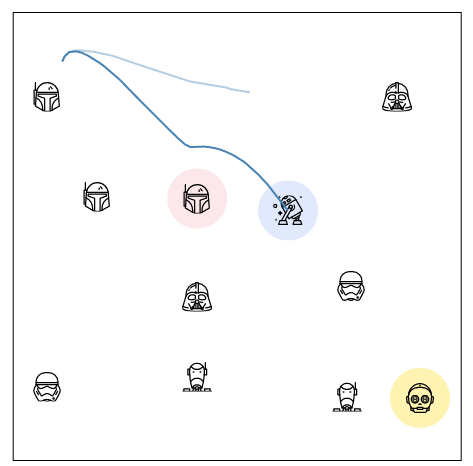
\includegraphics[width=0.8\linewidth, height=0.8\linewidth]{img/sim2b.png}
  \caption{Blackbox Beispiel mit veränderbaren Parametern}
  \label{fig:sw_blackbox}
\end{figure}

Nach der Erklärung des Beispiels folgt eine Überleitung zum theoretischen Teil. In dieser Überleitung ("Der Algorithmus") wird der Nutzer noch einmal darauf hingewiesen, dass die \textit{Potential Fields Method} einen physikalischen Hintergrund hat und wie der Zusammenhang zu den Objekten in der Abbildung ist.
Der Nutzer wird erst an dieser Stelle explizit auf die Möglichkeit aufmerksam gemacht, dass die Einstiegsabbildung eine interaktive Animation (Abbildung \ref{fig:sw_blackbox}) ist. Der Nutzer kann diese starten, pausieren und fortsetzen, die Objekte verschieben und so neue Szenarien kreieren. Der zurückgelegte Pfad von R2D2 wird als blaue Linie visualisiert. Sobald R2D2 seinen Freund C3PO erreicht, startet die Animation von vorne. Der alte Pfad wird transparenter dargestellt, um den Unterschied zu einem neuen Szenario zu verdeutlichen. Dies ist darauf begründet, dass ein Nutzer sich den Unterschied nicht merken muss und dadurch verständlicher wird ("Eye over Memory" \cite{munzner2015visualization}).

Wir haben diesen Blackbox-Ansatz gewählt, um das Verständnis über das beschriebene Beispiel durch die interaktive Animation zu festigen. Dem interessierten Nutzer stellen sich nun Fragen bezüglich des Algorithmus, vor allem, wie die \textit{Potential Fields Method} funktioniert.

In dem Abschnitt "Parametererklärung" wird der Algorithmus im Whitebox-Verfahren erklärt, d.h. der Nutzer wird nun mit mathematischen Formel und deren Auswirkungen konfrontiert. Die vorherige Animation wird durch ein simpleres und nicht veränderbares Szenario ersetzt (Abbildung \ref{fig:sw_whitebox}). 
%\begin{figure}[h!]
%  \centering
%  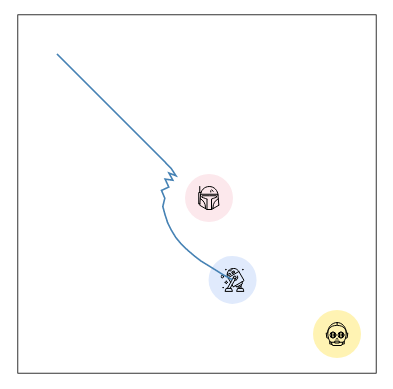
\includegraphics[width=0.7\linewidth, height=0.7\linewidth]{img/sim1.png}
%  \caption{Whitebox Beispiel mit veränderbaren Parametern}
%  \label{fig:sw_whitebox}
%\end{figure}
Das Szenario zeigt nun die Roboter R2D2 und C3PO und einen Gegner. R2D2 muss nur noch ein Hindernis umfahren, wodurch die folgende Erklärung mit ihren mathematischen Formeln anschaulicher vermittelt werden kann.

Die grundlegende Formel \ref{eq:grad_field} und die zwei Terme (Formel \ref{eq:grad_attr} und \ref{eq:grad_rep}) werden beschrieben.
Um das Verständnis der Potentialfelder zu veranschaulichen dienen sogenannte Surface Plots. Die Surface Plots sind so gewählt, dass sie das Szenario abbilden. Das anziehende Potentialfeld (Abbildung \ref{fig:surf_attr}) kann als Abhang verstanden werden, wobei das Tal das Ziel und das Gefälle die Anziehungskraft darstellt.
\begin{figure}[h!]
  \centering
  \fbox{
  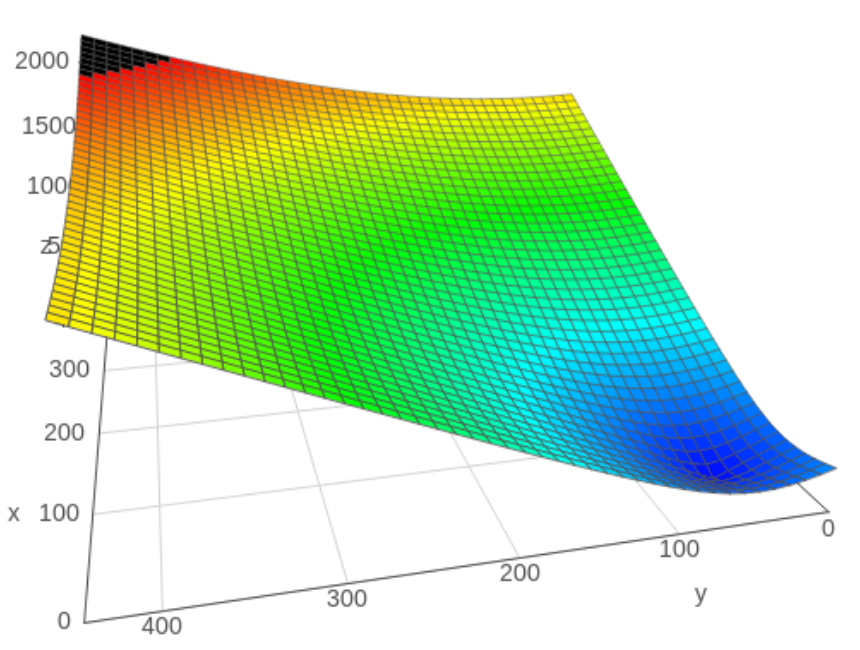
\includegraphics[width=0.8\linewidth, height=0.8\linewidth]{img/attr.png}}
  \caption{Das anziehende Potential}
  \label{fig:surf_attr}
\end{figure}
Der Nutzer hat die Möglichkeit über einen Regler den Parameter $\epsilon$ (Formel \ref{eq:pot_attr}) zu verändern und sieht unmittelbar die Auswirkungen im Surface Plot und im Szenario. 
Das Potentialfeld für die abstoßende Kraft und den Einflussbereich des Hindernisses kann als Berg auf einer Ebene verstanden werden (Abbildung \ref{fig:surf_rep}). Die Parameter $\theta$ und $\phi$ (Formel \ref{eq:pot_rep}) können ebenfalls über Regler angepasst werden. Auch hier sind die Auswirkungen im Surface Plot und im Szenario sichtbar.
\begin{figure}[h!]
  \centering
  \fbox{
  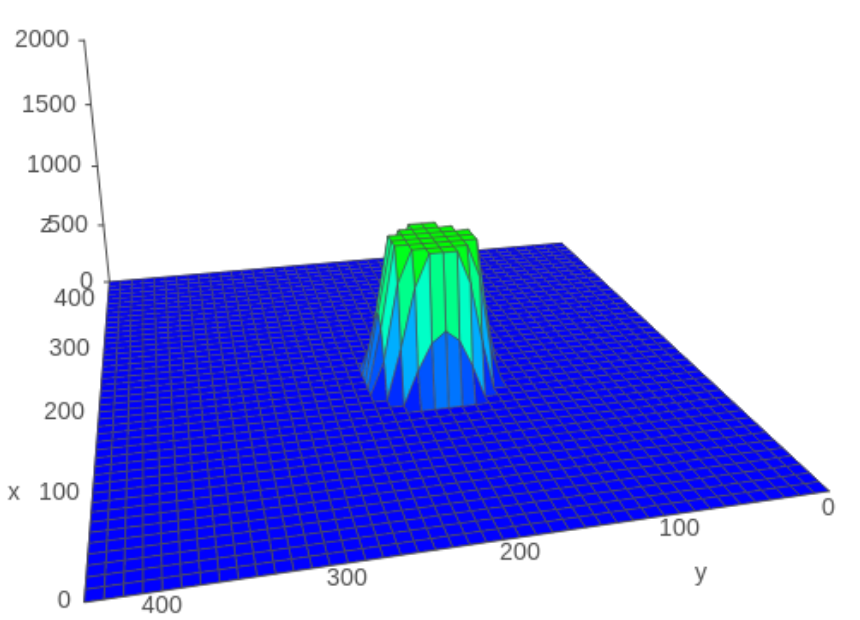
\includegraphics[width=0.8\linewidth, height=0.8\linewidth]{img/rep.png}}
  \caption{Whitebox Beispiel mit veränderbaren Parametern}
  \label{fig:surf_rep}
\end{figure}
Zum Abschluss der Erklärung wird die Kombination von anziehendem und abstoßendem Potentialfeld visualisiert (Abbildung \ref{fig:surf_pot}).
%\begin{figure}[h!]
%  \centering
%  \fbox{
%  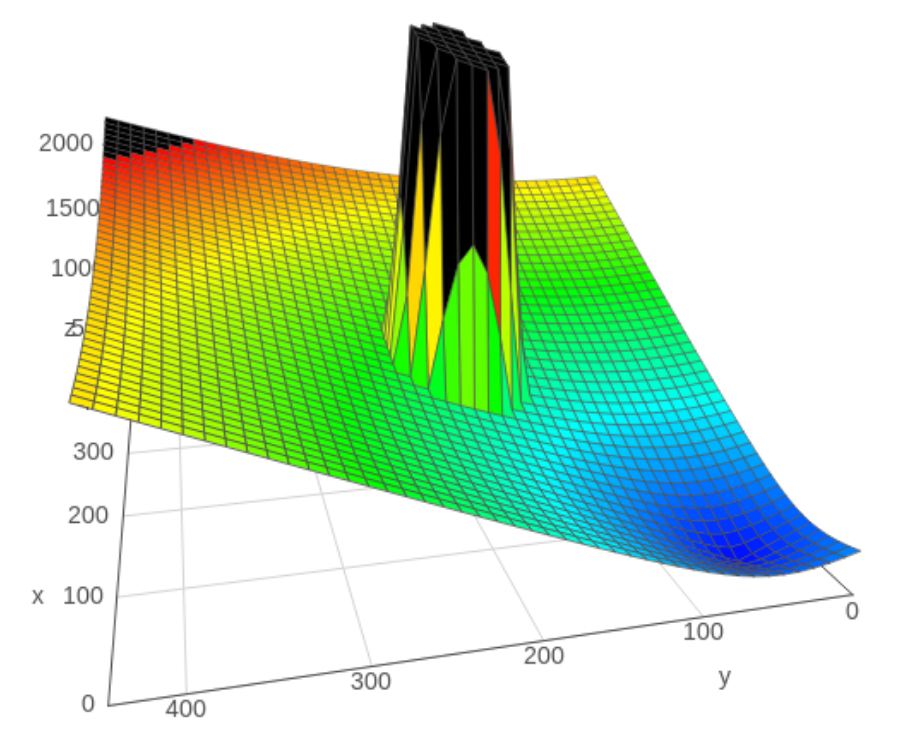
\includegraphics[width=0.7\linewidth, height=0.7\linewidth]{img/pot.png}}
%  \caption{Whitebox Beispiel mit veränderbaren Parametern}
%  \label{fig:surf_pot}
%\end{figure}

Surface Plots und Szenario werden nebeneinander angezeigt  (Abbildung \ref{fig:combi}).
Der Unterschied zu einem vorherigem Durchlauf der Animation wird auch hier durch eine transparentere blaue Linie visualisiert. Zusätzlich wird die Erklärung für die rote Markierung der Gegner erklärt. Diese spiegelt das nächstliegende Hindernis von R2D2 dar. 
Die gewählten Surface Plots sind keine neue Visualisierung für Potentialfelder. Wir haben sie dennoch gewählt, da die Surface Plots sehr anschaulich die Potentiale vermitteln. Im Gegensatz zu den Beispielen \ref{fig:other_pyrob}, \ref{fig:other_mcgill} und \ref{fig:other_elec} benötigt der Nutzer keine Vorkenntnisse zum Interpretieren von Vektorfeldern, Farbkarten oder elektrischen Feldern. Die Analogie der Potentialfelder zu Tal und Berg ist intuitiv und leicht verständlich.
Darüber hinaus soll die Gegenüberstellung und gleichzeitige Verknüpfung von Surface Plot und Szenario das Verständnis fördern.

\begin{figure*}
\centering
\begin{minipage}[t]{.48\textwidth}
\centering
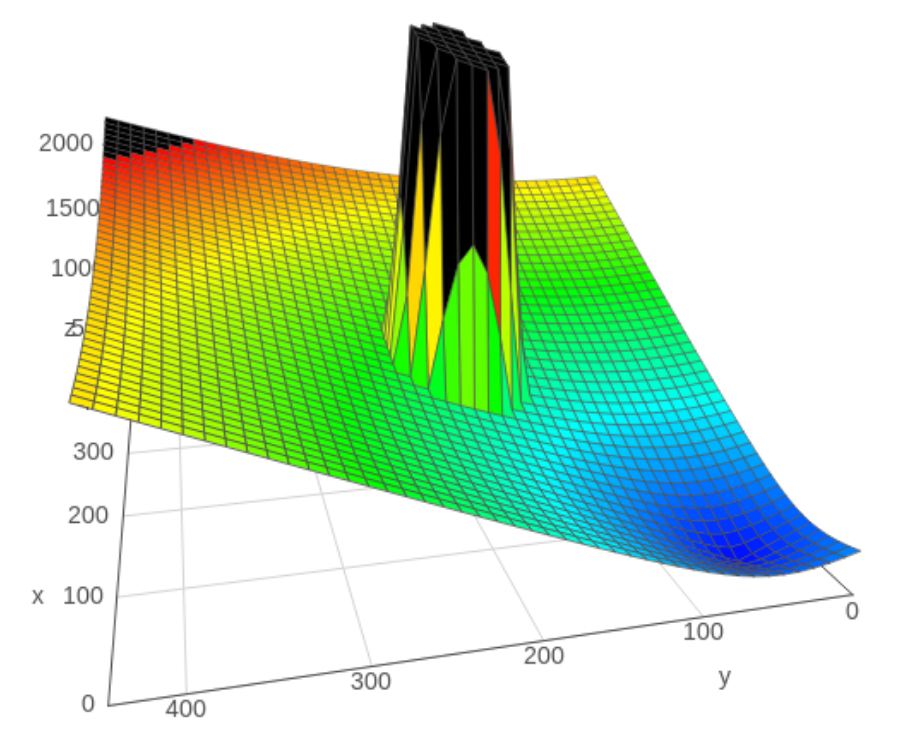
\includegraphics[width=0.8\linewidth, height=0.8\linewidth]{img/pot.png}
\caption{Das Potentialfeld: anziehendes und abstoßendes Potentialfeld}\label{fig:surf_pot}
\end{minipage}\hfill
\begin{minipage}[t]{.48\textwidth}
\centering
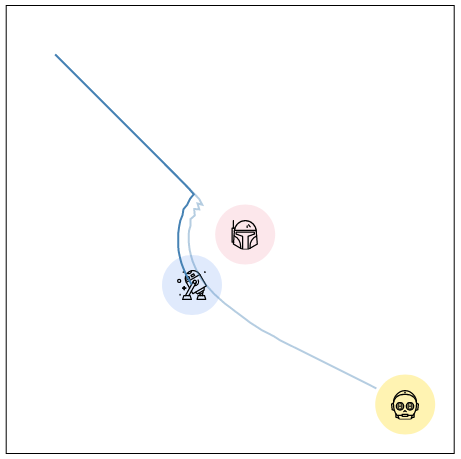
\includegraphics[width=0.8\linewidth, height=0.8\linewidth]{img/sim1b.png}
\caption{Whitebox Beispiel mit veränderbaren Parametern}\label{fig:sw_whitebox}
\end{minipage}
\caption{Potentialfelder und Szenario werden nebeneinander dargestellt}
\label{fig:combi}
\end{figure*}

Am Ende des Projekts kann der Nutzer alle Parameter auf die ursprüngliche Animation anwenden und die Auswirkungen auf verschiedene, selbst erzeugte Szenarien sehen. Dabei wird er zwangsläufig auf Limitierungen des Algorithmus aufmerksam. Weitere Informationen werden über eine Weiterleitung auf andere Seite bereitgestellt.
%TODO Limitierungen in IdyllPage einbauen (Vermerk oder Fragestellung).

\subsection{Differenz zum Prototyp}
Unsere Implementierung hat ein paar Differenzen zum Prototyp.
Da bei unserem Cognitive Walkthrough (\vref{sec:cogWal}) uns ein paar Unstimmigkeiten aufgefallen sind, haben wir sie sogleich verbessert.
\begin{itemize}
	\item Aufmerksamkeitsfluss: Wir haben den Aufmerksamkeitsfluss verändert, sodass die Simulation nicht von Anfang an spielt, sondern durch den Text gestartet werden muss. Da dies in der Presentation auf Kritik stoß, weil dieses Konzept didaktisch zu streng sei, haben wir zusätzlich noch einen Steuerknopf eingefügt. Dieser Knopf wird erst sichtbar, wenn der Nutzer etwas nach unten scrollt. Dadurch kann die Simulation auf intuitive Art auch ohne das Lesen des Textes gesteuert werden.
	\item Metapher: Wir haben uns für eine Star Wars-Metapher entschieden, da diese Filme eine breite Zuschauerschaft haben und die Metapher somit allgeimein verständlich sein sollte. Diese Metapher haben wir auch bei der Erklärung im Text aufgegriffen.
	\item Die Veränderung des Pfads durch das Benutzen von Parametern wurde aus der 3D-Abbildung genommen und in die Star Wars-Metapher verlagert. Die 3D-Abbildung und die Beibehaltung der Star Wars-Metapher ermöglichen einen kontinuierlichen Erzählstrang der Seite.
	\item Die Darstellung der Isokonturen mit lokalen Vektorfeldern wurde weggelassen, da sie unserer Ansicht nach die Seite zu sehr überlädt und keinen verbesserten Nutzen zur Erklärung beiträgt. Auch hier kam der berechtigte Vorschlag, diese zusätzliche Ansicht in das Star Wars-Beispiel zu integrieren, welche über einen Steuerknopf aktiviert/deaktiviert werden kann. In einer nächsten Version wäre über eine Implementierung nachzudenken.
	\item Der Hinweis auf Probleme des Algorithmus werden nur noch mit einer Frage angedeutet. 
	\item Ursprünglich hatten wir noch das Einfügen von mehr Hindernissen und dynamisch bewegliche Hindernisse angedacht. Allerdings hatten wir in Hinblick auf unsere Zeitplanung diese nur als Optionen vorgemerkt. Wie sich herausgestellt hat, haben wir die Zeit an anderer Stelle benötigt (Insbesondere Schwierigkeiten mit Idyll stellten sich als schwerer als gedacht dar.)
\end{itemize}

% =============================================================================
\section{Evaluation}
% =============================================================================
%TODO hier müssen wir unbedingt noch was reinschreiben


\subsection{Cognitive Walkthrough}\label{sec:cogWal}
Wir haben nach einer ersten Implementierung in der Gruppe einen Cognitive Walkthrough gemacht. Dabei haben wir die folgendende Punkte bemerkt:
\begin{itemize}
	\item Die abstrakte Darstellung der Objekte im Prototyp lädt nicht sehr zum Lernen ein. Es braucht eine gute Metapher um den Algorithmus und das Problem interessant zu machen.
	\item Statische Blackbox: Die statische Blackbox hat die Aufmerksamkeit durch die Animation sehr stark angezogen. Keiner von uns hatte noch Lust den Text zu lesen. Stattdessen haben wir die Simulation gestartet und nur noch dem Roboter zugeschaut. Danach sind wir lieber zur nächsten Visualisierung übergegangen.
	\item Whitebox: Das gleichzeitige Anzeigen von Erklärungstext, Surface Plot, Isokonturen mit Vektordarstellung und Beispiel-Szenario haben den einfachen und klaren Aufbau der Seite gestört. Sie war an dieser Stelle zu überladen.
	\item Limitierungen: Durch das Erstellen von eigenen Szenarien, kann der Nutzer zügig auf diese stoßen. Für ein tiefer gehendes Verständnis muss sich der Nutzer noch detaillierter mit der \textit{Potential Fields Method} und ihren Variationen beschäftigen. Für einen ersten Einstieg in die Robotik fanden wir die subtile Andeutung auf Limitierungen des Algorithmus didaktisch sinnvoller, da Informatikstudenten und -studentinnen immer über Grenzfälle und Probleme von Algorithmen nachdenken sollten. Das bloße hinnehmen von Lösungen fördert nicht die Kritikbereitschaft, die in einigen Fällen angebracht wäre.
\end{itemize}

\subsection{Tester}
Wir haben verschiedene Gruppen getestet:


Informatik-Studierende (über 3. Semester):
\begin{itemize}
	\item Verständlich dank Animation
	\item Animation war anschaulich
	\item Parameter spielen war gut
	\item Star Wars ist eine gute Metapher
	\item Animation zu den Kräften % Eh, What?
	\item Parametererklärung könnte besser unterteilt werden
\end{itemize}

Informatik-Studierende (1.-3. Semester):
\begin{itemize}
	\item Lokale Minima wurden selbstständig als Problem erkannt
	\item Reset-Button für eine bessere Steuerung der Simulation wurde gewünscht
	\item Statistiken in der Simulation (Zurückgelegter Weg, benötigte Zeit zum Ziel) würden eine noch spielerische Atmosphäre erzeugen
	\item Motivation durch spielen
\end{itemize}

Informatik-Studierende (Abitur):
\begin{itemize}
	\item Griechische Buchstaben sind angsteinflößend
	\item Mathematik wirkt immer noch abschreckend
	\item Idee des Algorithmus wird klar
	\item Simulation hilft bei Verständnis
	\item Hinderniseinflussbereich in der Simulation wird missverstanden
	\item Metapher wurde verstanden
\end{itemize}
%Flip:
% Hat lokal minima problem herausgefunden
% Reset-Button waere gut
% Fancy statistiken in simulation

% =============================================================================
\section{Fazit}
% =============================================================================
%Abgleich mit Zielen
%Was haben wir erreicht?
Wir konnten innerhalb der vorgesehenen Zeit einen Prototypen entwickeln.
Zur Presentation am 14.02.2019 konnten wir den Prototypen presentieren und in der Zeit bis zur Paperabgabe noch das Feedback der Presentation einarbeiten.
Dabei ist es uns gelungen eine leicht verständliche Metapher für das Problem zu finden und einzusetzen. 
Wir haben beim Cognitive Walkthrough nach einer ersten Implementierung auch Schwächen des Prototyps gefunden. 
Die Schwächen haben wir verbessert und die Änderungen vermerkt.

%Wie waren die Testergebnisse?
Die Tester haben ab dem dritten Semester haben sehr gut auf unsere Seite reagiert. Allerdings sind sie nicht Teil der Zielgruppe, deshalb überzeugt uns dieses Feedback nur von der inhaltlichen Richtigkeit unserer Applikation.

In der Kategorie der 1.-3. Semester-Studierenden %TODO Auswertung tests

%Was haben wir gelernt?
%Was wuerden wir anders machen?
Während des Projekts ist uns klar geworden, dass wir mit dem Prototypen deutlich mehr Evaluierung hätten machen sollen. 
Dadurch wären die Schwächen, die im Cognitive Walkthrough zu Tage kamen deutlich früher erkannt worden.
Daher würden wir bei unserem nächsten Projekt deutlich mehr auf diesen Schritt achten.


%Wo ist das Video und die Seite?



\bibliographystyle{ACM-Reference-Format}
%\bibliography{sample-bibliography}
\bibliography{sample-bibliography.bib}

\end{document}
